\documentclass{text-style}

\texttitle{Визуальные языки и их использование в IDE}

\begin{document}

\maketitle
\thispagestyle{empty}

\section{Введение}

% Слайд 1.
Хочу представить вашему вниманию краткий обзор текущего положения дел в визуальных языках как инструментах разработки, в частности, их использовании в современных IDE. Начнём с того, зачем визуальные языки вообще.

Всерьёз работать с визуальными языками начали где-то в начале 1970-х годов, прежде всего в крупных оборонных проектах США, когда внезапно оказалось, что стоимость разработки программного обеспечения вполне может оказаться больше стоимости всего остального, при этом сроки реализации совершено непредсказуемы. На визуальные языки возлагались надежды, что они по аналогии с чертежами в <<обычной>> инженерии смогут сделать разработку ПО более управляемой. К началу 90-х годов надежды на визуальные языки достигли пика: люди верили, что программы можно будет просто рисовать, собирая из готовых блоков и соединяя на диаграмме связями, после чего генерировать работающий код. Первые успехи во внедрении инструментов визуального проектирования (тогда их называли <<CASE\footnote{Computer-Aided Software Engineering}-системы>>) этому сильно способствовали, стали говорить даже, что визуальные языки имеют перспективы стать <<языками четвёртого поколения>>, давая выигрыш в разы производительности труда по сравнению с текстовыми языками, как в своё время языки высокого уровня произвели революцию и вытеснили ассемблер. В те же времена (в 1995-м году) появился язык UML, как объединение наиболее популярных тогда методологий визуального моделирования. И Rational Unified Process, методология разработки вокруг визуальных моделей на UML. 

А потом наступила эра Agile и программистское сообщество с визуальными языками стало активно бороться. Отчасти потому, что визуальное моделирование воспринималось как основной атрибут тяжеловесных методологий, давящих творческие начинания программистов в грудах документации и подробно специфицированных процессах. Отчасти потому, что революции и нового поколения языков так и не случилось --- визуальные методологии лет 15 находились в состоянии <<ещё чуть-чуть, и все начнут программировать визуально>>, так что даже самые верные апологеты визуальных языков потеряли веру. 

% Слайд 2.

Сейчас, по несколько субъективным ощущениям, в целом по индустрии ситуация с визуальными языками в разработке такая:

\begin{itemize}
    \item ряд крупных компаний не использует визуальные модели вообще\footnote{Как говорили мне когда-то коллеги из Yandex, у них сколько-то гигабайт кода и ни одной UML-диаграммы.};
    \item в open-source-проектах визуальные модели, да и внятная архитектурная документация вообще, существует практически только в проектах-примерах для курсов по архитектуре\footnote{Некоторое подтверждение этому --- книга <<The Architecture of Open Source Applications>>, URL: \url{http://aosabook.org/} (дата обращения: 25.12.2022), состоящая из статей об архитектуре известных проектов от их авторов или maintainer-ов; ровно три статьи из 49, представленных в книге, содержат корректные UML-диаграммы.};
    \item однако есть и компании, целиком строящие процесс разработки вокруг UML, но таких меньшинство --- в основном в области mission-critical ПО, например, военного (не раз встречал упоминания о разных вариациях ДРАКОН\footnote{Дружественный Русский Алгоритмический язык, Который Обеспечивает Наглядность --- по сути, сильно продвинутые блок-схемы.} в этой сфере, например);
    \item сам стандарт UML не обновлялся с 2017 года;
    \item однако вполне живо предметно-ориентированное визуальное моделирование, и сейчас, после некоторой потери интереса в 2010-х, про него слышно всё чаще. Предметно-ориентированные языки вызывают живой интерес у <<непрофильной>> индустрии --- к нам иногда обращаются крупные не-IT-компании с просьбами, связанными с предметно-ориентированными языками.
\end{itemize}

% Слайд 3.

\section{Предметно-ориентированное моделирование}

Поговорим подробнее про предметно-ориентированное моделирование. Основная идея его в том, что визуальный язык создаётся под конкретную предметную область или даже задачу, а не пытается служить универсальным языком программирования (в качестве аналога в мире текстовых языков можно привести SQL). Это позволяет:

\begin{itemize}
    \item генерировать исполнимый код, потому что генератор <<знает>>, для чего конкретно этот код и с чем будет работать;
    \item сделать сам язык понятным для людей, знакомых с предметной областью.
\end{itemize}

Последнее свойство особенно важно, поскольку позволяет программировать людям, которые программировать не умеют. Например, в образовательной робототехнике визуальные языки программирования роботов (например, в системе Robolab или нашей разработке TRIK Studio) успешно применяются с начальной школы, когда дети не умеют даже ещё читать. Развитие <<интернета вещей>>, доступные облачные ресурсы возродили интерес к предметно-ориентированным языкам, в контексте <<программирования конечным пользователем>> (end-user programming), или того, что называют модным термином <<low-code/no-code solution>>. Это довольно сильно отличается от традиционного понимания визуальных языков как языков программирования следующего поколения, но не раз доказало свою полезность. Интересные примеры таких систем --- визуальный язык Unreal Engine (<<Blueprint>>), язык веб-программирования Webflow Logic, система программирования роботов Microsoft Robotics Developer Studio, среды образовательного программирования роботов Robolab, NXT-G, TRIK Studio.

% Слайд 4.

\section{DSM-платформы}

Однако разработка визуальных редакторов --- дело дорогое и сложное. Делать свой редактор под каждую задачу крайне неэффективно, поэтому с начала 1990-х годов ведутся серьёзные теоретические исследования в области формального задания синтаксиса (а иногда и семантики) визуального языка, и автоматической генерации инструментов для работы с языками по этому описанию. Есть несколько известных примеров систем, которые так умеют --- MetaEdit+, Eclipse Graphical Modeling Project\footnote{На самом деле, это <<зонтичный>> проект, включающий в себя как набор библиотек, так и несколько инструментов, которые пользуются библиотеками, чтобы реально что-то делать с языками --- например, Eclipse Sirius (\url{https://www.eclipse.org/sirius/}).}, и ещё куча не очень известных, например, наша разработка QReal\footnote{https://github.com/qreal/qreal (дата обращения: 25.12.2022)}. Такие системы называются DSM-платформами (или, раньше, MetaCASE-инструментами), и являются аналогами генераторов синтаксических анализаторов наподобие ANTLR, но для визуальных языков. Для текстовых языков, кстати, есть более близкий аналог --- JetBrains MPS.

% Слайд 5.

\section{Формальное задание языков}

Визуальные языки описываются в основном с помощью метамоделирования. Метамодель --- это, как правило, визуальная модель, которая описывает множество корректных моделей. Метамодели описывают сущности в языке, их атрибуты с типами, правила связи между сущностями. Метамодель сродни грамматике для текстовых языков, и некоторые визуальные языки даже пытались задавать графовыми грамматиками, но это как-то не прижилось. Стандарт UML описывает язык именно в терминах метамоделей, причём, что интересно, сначала формально описывает метамодель в терминах самой метамодели, старательно избегая круговых зависимостей --- метаязык по сути тоже визуальный язык, значит может быть выражен сама на себе. У UML метаязык --- по сути сильно упрощённая диаграмма классов\footnote{Есть ещё MOF (Meta-Object Facility), его часто путают с метаязыком, на котором описан UML. Это почти правда, MOF --- это отдельная и слегка расширенная версия метаязыка UML.}. Вот рисунок с примером:

% Слайд 6.

\begin{center}
    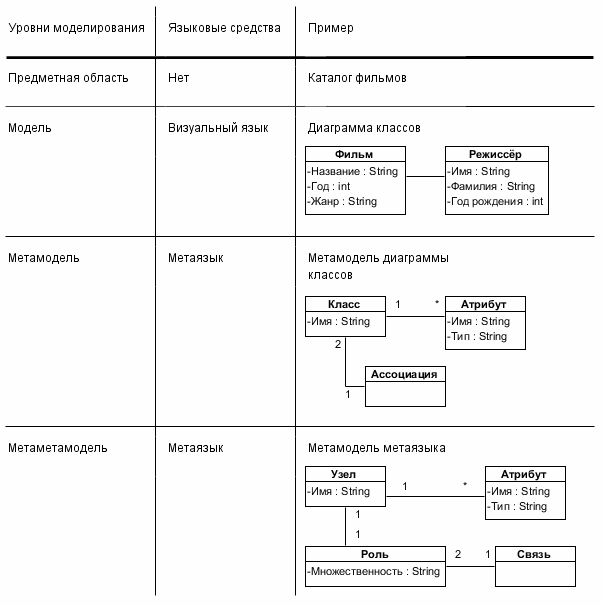
\includegraphics[width=0.6\textwidth]{metalevels-ru.png}
\end{center}

Предметная область моделируется диаграммой классов, которая, в свою очередь описывается диаграммой <<классов>>, где вводятся понятия <<Класс>>, <<Атрибут>> и т.п. --- то есть метамоделью диаграммы классов. Которая сама есть диаграмма на метаязыке, который описывается своей метамоделью (называемой <<метаметамодель>>). Метеметамета- и т.д. -моделей не бывает, потому что любой нормальный метаязык должен уметь описывать сам себя.

% Слайд 7.

Внешне всё выглядит просто, но дьявол в деталях. Например, в UML есть и диаграмма классов, и диаграмма объектов. В примере выше у класса <<Фильм>> на диаграмме объектов может быть экземпляр, конкретный фильм (например, <<Терминатор>>). Можно было бы подумать, что конкретный фильм должен быть на уровне предметной области, но нет: диаграмма объектов --- это диаграмма, часть модели, так что <<Терминатор>> находится на уровне <<Модель>> на рисунке, и формально, с лингвистической точки зрения, с <<Фильм>> никак не связан, и тот факт, что он обязан, например, иметь атрибуты <<Название>>, <<Год>> и <<Жанр>> в метамодели UML никак не выразить. А следовательно, как-то автоматически проверять корректность диаграмм в инструментах тоже не получится --- приходится реализовывать нестандартные ad-hoc-решения.

Чтобы с этим бороться, придумали формализмы <<многоуровневого>> и <<глубокого>> метамоделирования, где любая модель, являясь экземпляром своей метамодели, может выступать в роли метамодели для моделей более низкого уровня, и так несколько раз. В глубоком метамоделировании диаграмма объектов была бы <<честным>> экземпляром диаграммы классов. Этот подход предлагали комитету по стандартизации UML ещё при подготовке UML 2.0, но изменения сочли слишком революционными и отвергли, поэтому глубокое метамоделирование и UML до сих пор развиваются независимо (точнее, UML уже особо не развивается). Из инструментов, поддерживающих формализм глубокого метамоделирования, стоит отметить Melanee (инструмент от авторов и главных евангелистов подхода), REAL.NET (потому что мы его делали, хотя он так и остался очень исследовательским проектом).

% Слайд 7.

\section{Визуальные языки в IDE}

Однако вернёмся к использованию средств визуального моделирования в разработке, а конкретно --- в IDE. Поскольку в современных IDE средства рисования диаграмм играют второстепенную роль, а хороший инструмент рисования диаграмм по сложности и стоимости легко превзойдёт даже очень хороший текстовый редактор, в IDE применяют два принципиальных подхода к поддержке диаграмм.

\begin{itemize}
    \item Взять готовую библиотеку для рисования диаграмм и сделать поверх неё ad-hoc-решение, поддерживающее только самые популярные диаграммы, но хорошо интегрирующее их с кодом. Пример IDE, которая пошла по такому пути --- IntelliJ IDEA, которая использует библиотеку yFiles для рисования. Вариант такого подхода --- вообще не поставлять <<из коробки>> поддержку диаграмм, надеясь на сообщество и интеграцию с существующими инструментами. Например, по такому пути пошла Visual Studio Code, предоставляя силами сообщества интеграцию с Diagrams.net --- вполне годным редактором диаграмм, умеющем, в том числе, и UML. На самом деле, Diagrams.net (ранее draw.io) создавался как демонстрационный прототип для библиотеки mxGraph\footnote{\url{https://jgraph.github.io/mxgraph/}.}, но дело пошло и он стал стандартом де-факто в веб-рисовании диаграмм (на мой вкус это плохая новость для сообщества, потому что при всех его достоинствах Diagrams.net --- просто векторный редактор, про синтаксис или семантику визуальных языков он ничего не знает). Ни yFiles, ни даже Diagrams.net формальный синтаксис UML не умеют (хотя Diagrams.net довольно неплохо мимикрирует).
    \item Попытаться разработать свою DSM-платформу, чтобы потом поверх неё реализовать поддержку любых языков визуального моделирования, в том числе и <<самодельных>>. По такому пути пошли Eclipse и Visual Studio. 
    \begin{itemize}
        \item Eclipse, поскольку с открытым исходным кодом, и популярная в своё время IDE, привлёк внимание научного сообщества, которое написало для него целую кучу инструментов в рамках проектов EMF (Eclipse Modeling Framework) и GMP (ранее GMF --- Graphical Modeling Framework). GMP использует несколько упрощённое по сравнению с UML задание метамодели (и изначально в XML или в виде классов на Java, хотя потом для него и графические метаязыки сделали), однако умеет очень и очень многое. GMP стал стандартом де-факто в исследовательских проектах по визуальным языкам, с тысячами (в буквальном смысле) контрибьюторов, на нём делают и поддержку UML, и прототипы с глубоким метамоделированием, и более экзотические экспериментальные среды. Однако проект большой и сложный, и поскольку над ним работает много исследовательских коллективов, любая информация, которую по нему можно найти, скорее всего, уже устарела. Собрать что-то боеспособное на Eclipse GMP требует много труда и знаний. Немного помогают проекты типа Sirius, которые объединяют в продуктовом виде возможности библиотек. Ещё субъективный недостаток этой платформы --- характерно староватый и страшноватый пользовательский интерфейс Eclipse.
        \item Для Visual Studio разрабатывалась Microsoft Domain-Specific Language Tools (MS DSL Tools, сейчас Modeling SDK for Visual Studio), относительно полноценная DSM-платформа, позволяющая в теории создавать произвольные визуальные языки и запускать их как плагины к Visual Studio. Microsoft серьёзно подошла к продуктовой стороне дела, даже издала книгу S.Cook et al, <<Domain-Specific Development with Visual Studio DSL Tools>>, включала DSL Tools в инсталлятор (правда, как опциональный компонент, по умолчанию не ставился). Дело не пошло, и сейчас Modeling SDK поддерживается, но, насколько можно судить, активно не развивается. Почему --- как часть платной среды разработки он не стал популярен в научном сообществе, как самостоятельная DSM-платформа он слабоват (например, там странный иерархический способ задания метамодели, неочевидно, как выразить циклические зависимости между сущностями). Однако, насколько слышал автор, существующая в Visual Studio поддержка визуального моделирования --- это на самом деле сильно переработанные DSL Tools (точнее, ещё до публикации DSL Tools кодовые базы разделились, и для Visual Studio на базе существовавших тогда наработок делали что-то специализированное).
    \end{itemize}
\end{itemize}

% Слайд 8.

Особенность использования визуальных языков в IDE --- необходимость интеграции с кодом в текстовом виде, чтобы редактирование диаграммы и текста было согласовано. Для Eclipse это долгое время было большой научной проблемой, потому что GMP существовал несколько отдельно от средств IDE для работы с текстом, и там пытались решать эту задачу в общем виде --- при произвольных изменениях на диаграмме и в тексте (даже вне IDE). Получалось плохо, потому что в общем виде это требует хитрых эвристик, и даже человек далеко не всегда может сказать, что поменялось, что удалилось, что добавилось. В IDEA и Visual Studio, насколько можно судить, инструменты для работы с диаграммами используют объектное представление кода (то, что называется в IDEA PSI, Program Structure Interface), так что диаграммы и текстовый код --- по сути просто виды на единую внутреннюю модель кода, так что синхронизировать изменения им гораздо проще, чем другим инструментам.

Общее слабое место всех редакторов диаграмм, как встроенных в IDE, так и отдельных --- это Usability. Субъективно лучший в этом плане --- десктопная версия Visual Paradigm, однако студенты, которым впервые предлагается рисовать на нём диаграммы на курсе по архитектуре, поначалу довольно негативно на него реагируют. Субъективно лучший из веб-редакторов --- diagrams.net, однако он весьма неинтуитивен и в целом довольно неудобен в использовании.

% Слайд 9.

\section{Визуальные языки в СПбГУ}

Наконец, кратко расскажу об опыте СПбГУ в разработке инструментов для визуального моделирования.

\begin{itemize}
    \item Первые работы по визуальному моделированию выполнялись ещё Андреем Николаевичем Тереховым в 80-х годах, для программирования телекоммуникационного оборудования. Впоследствии эти работы превратились в технологию RTST, которая эволюционировала в RTST++. В этих работах использовался язык SDL (до сих пор любимый в телекоммуникационных кругах), генерация кода в Алгол-68. Поскольку вся технология, включая транслятор Алгол-68, также разрабатывалась в СПбГУ, выбранный подход интеграции текстового и графического программирования был похож на то, что применяется в Visual Studio и IDEA --- среда <<понимала>> и текст, и диаграммы, и позволяла эффективно генерировать код со вставками на Алгол. 
    \item REAL стал продуктом эволюции RTST, его последняя <<итерация>> --- REAL-IT, был написан уже на C++ и генерировал код, в частности, в Visual Basic. С его помощью был разработан ряд информационных систем для студотдела математико-механического факультета СПбГУ, причём по канонам модельно-ориентированной разработки --- большая часть системы моделировалась и генерировалась, почти ничего не писалось вручную.
    \item Примерно в 2003 году REAL-IT перестал поддерживаться, возникла некая пауза, после которой в 2007 году появился QReal как, поначалу, попытка сделать кроссплатформенный REAL-IT на современных для того времени технологиях и поддерживавший только недавно тогда появившийся стандарт UML 2. Однако стало быстро понятно, что поддерживать все языки из UML вручную на C++ --- слишком много работы, поэтому авторы начали экспериментировать с генерацией редакторов по описанию языка, что в итоге привело к созданию полноценного метаредактора и визуального метаязыка. Благодаря этому на QReal было сделано сразу несколько экспериментальных технологий, однако, что интересно, UML так и не был полностью поддержан.
    \item Благодаря наличию метаредактора удавалось быстро (в течение недели-двух) отвечать на запросы <<сделайте мне такой-то визуальный инструмент>>, это позволило нам заинтересовать коллег с кафедры теоретической кибернетики и вместе с ними реализовать визуальный инструмент для образовательного программирования роботов QReal:Robots, примерно в 2011 году. Поначалу инструмент развивался медленно, хотя его и пытались применять в робототехнических кружках, однако с появлением робототехнического конструктора TRIK QReal:Robots получил финансовую поддержку и был переименован в TRIK Studio. 
    \item TRIK Studio до сих пор активно разрабатывается силами студентов математико-механического факультета и специалистов компании <<Кибертех>>, сейчас это одна из самых популярных в России сред образовательной робототехники. Архитектурно она всё ещё плагин к QReal, но кодовая база специфичной для робототехники части уже вполне сопоставима по объёму кода (если не превышает) всю остальную систему. TRIK Studio мы считаем самым успешным своим продуктом и примером возможностей правильно применённого визуального моделирования.
    \item Поскольку QReal/TRIK Studio стала большой <<промышленной>> системой, потребовался новый инструмент для быстрых экспериментов, так появился REAL.NET, примерно в 2016 году. Эта система была написана уже на .NET и изначально поддерживала многоуровневое метамоделирование, сначала это была десктопная система, потом была переписана под веб. На неё была сделана пара экспериментальных технологий, но из-за отсутствия интереса индустрии работа постепенно сошла на нет, и с лета 2022 года ничего нового в системе не делается.
\end{itemize}

% Слайд 10.

\section{Заключение}

Подведём краткие итоги доклада.

\begin{itemize}
    \item Визуальное моделирование после <<зимы>> 2010-х, кажется, снова вызывает интерес, прежде всего в контексте <<программирования конечным пользователем>>, и прежде всего в контексте предметно-ориентированных языков.
    \item Использование визуальных языков для промышленной разработки ограничено, поддержка их в IDE весьма ограниченна --- она присутствует практически везде, но везде имеет второстепенное значение.
    \item Возможности науки о визуальных языках в современных IDE недоиспользованы, в силу прохладного отношения вендоров, проистекающего из прохладного в целом отношения программистского сообщества к визуальным языкам.
    \item Настоящие диаграммы UML в среде разработки не поддерживает буквально никто (кроме Eclipse, где они используются в основном в отрыве от кода).
    \item Интегрированные в <<легковесные>> IDE low-code-решения могут быть интересным направлением развития инструментария и могут быть реально востребованы, как пример --- визуальный язык в Unreal Engine.
    \item Однако полноценный инструментарий создать сложно --- точнее, можно довольно легко сделать неудобный векторный редактор, а полноценную среду разработки с <<настоящими>> визуальными языками, да ещё и удобную, пока никто ещё не сделал, хотя многие пытались.
    \item Поэтому кажется, что подходить к проблеме надо основательно, и с двух сторон сразу --- как с точки зрения формализмов задания языков и порождения по ним инструментов, так и --- не менее важно --- с точки зрения usability редактора.
    \item При этом ad-hoc-решения скорее вредят делу, нужен переиспользуемый инструментарий.
\end{itemize}

\end{document}
